\section{Bayesian Neural Network}
As explained in \autoref{sec:bnn}, in order to handle uncertainty, Bayesian Neural Networks introduce a few changes, some of which were analyzed in this section. If not defined otherwise, the following assumptions were made:
\begin{itemize}
    \item the architecture used is a multilayer perceptron with 2 layers and a hidden size of $128$,
    \item the prior distribution is a scale mixture of two Gaussian densities \cite{Blundell2015} with a \textit{mixing coefficient} ($\pi$) equal to $0.5$, $\mu_1 = \mu_2 = 0$, $\sigma_1 = 1$ and $\sigma_2 = 1*10^{-6}$,
    \item learning was conducted for $20$ epochs, with batch size $64$ and Adam optimizer with learning rate of $1*10^{-3}$,
    \item a subset of $10000$ samples from the $28\textrm{x}28$ MNIST dataset was used.
\end{itemize}

\subsection{Learning process}
In the case of Bayesian Neural Networks, the learning process is rather similar to their conventional counterpart. While the loss function is counted differently (see \autoref{eq:bayes-by-backprop-loss}), it is minimized the same way as in conventional neural networks. Similarly, with other measures, such as \textit{accuracy} or \textit{F1}. In \autoref{fig:bnn-learning} sample graphs of loss and accuracy of BNN learning process were presented.

\begin{figure}[h]
     \centering
     \begin{subfigure}[b]{0.9\textwidth}
         \centering
         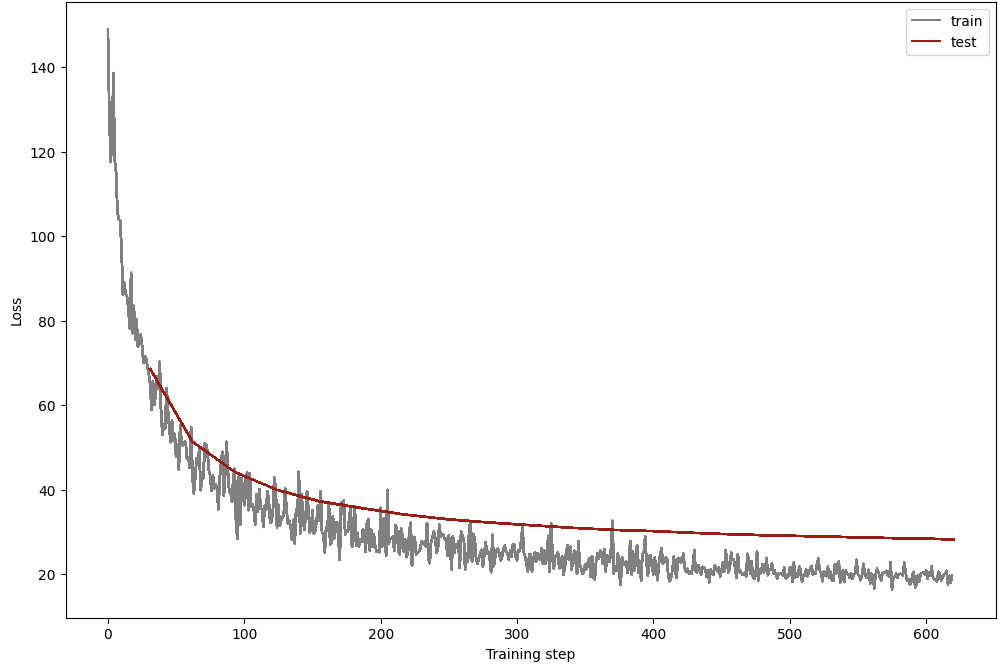
\includegraphics[width=\textwidth]{observational/img/bnn/bnn_loss.png}
         \caption{Loss over epochs}
         \label{fig:bnn-learning:loglikelihood}
     \end{subfigure}
     \begin{subfigure}[b]{0.9\textwidth}
         \centering
         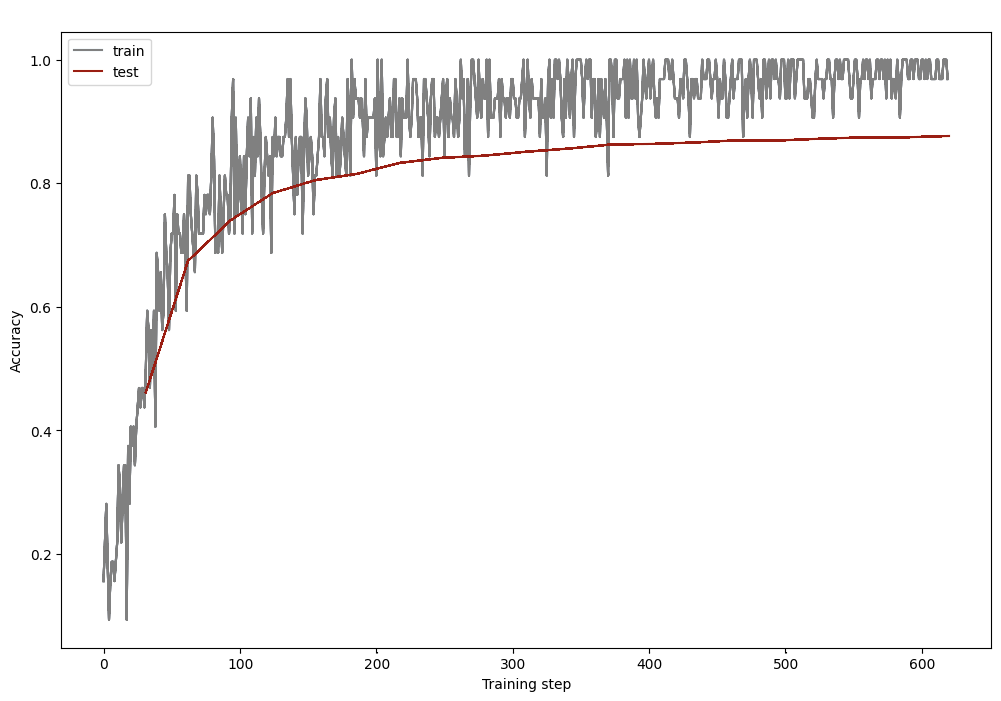
\includegraphics[width=\textwidth]{observational/img/bnn/bnn_acc.png}
         \caption{Accuracy over epochs}
         \label{fig:bpca-inference:elbo}
     \end{subfigure} 
     \caption[Loss and accuracy course during BNN learning]{Graphs show the Loss (a) and Accuracy (b) values over BNN model training epochs.}
    \label{fig:bnn-learning}
\end{figure}

\subsection{Uncertainty}
One of the most significant features of Bayesian methods is a possibility of reaching some level of explainability through uncertainty handling. In Bayesian Neural Networks, if distributions are applied over weights, it is possible to quantify confidence of the network in each of the predicted weights. In contrast to conventional neural networks (where a \textit{softmax} activation layer is used on non-probabilistic outputs to imitate this behavior \cite{Gal2016, Pearce2021}), uncertainty estimation is based on true probabilities.

\vspace{\baselineskip}
In \autoref{fig:bnn-uncertainty} an example uncertainty analysis was presented. It takes into consideration predicted classes, which are in fact extracted from the last layer only, because they are easily visualizable. Nevertheless, the same rules apply when measuring uncertainty for any of the layers, thus also any chosen representation. As a result of the Bayesian treatment, one can not only assess which classes the model confuses, but also to what extent. Additionally, sampling from a distribution allows for more robust and less computationally expensive evaluation. Because the inference in conventional neural networks is deterministic, only re-training the network multiple times would be equivalent to Monte Carlo draws in the Bayesian setting.

\begin{figure}[h]
     \centering
     \begin{subfigure}[b]{\textwidth}
         \centering
         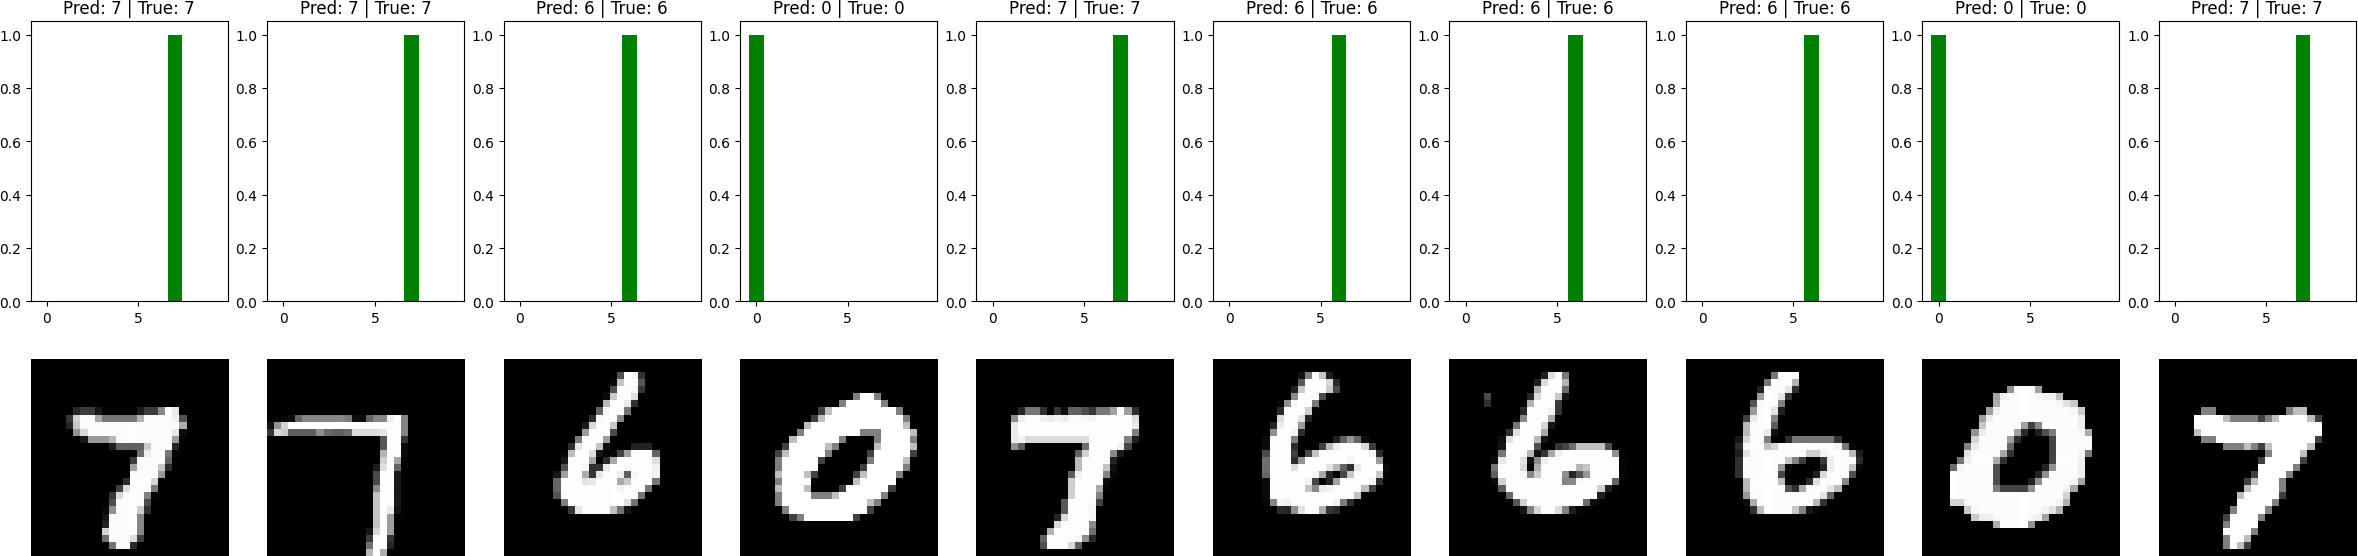
\includegraphics[width=\textwidth]{observational/img/bnn/bnn_top_high_correct.png}
         \caption{Top 10 high confidence correct predictions}
     \end{subfigure}
     \par\bigskip
     \begin{subfigure}[b]{\textwidth}
         \centering
         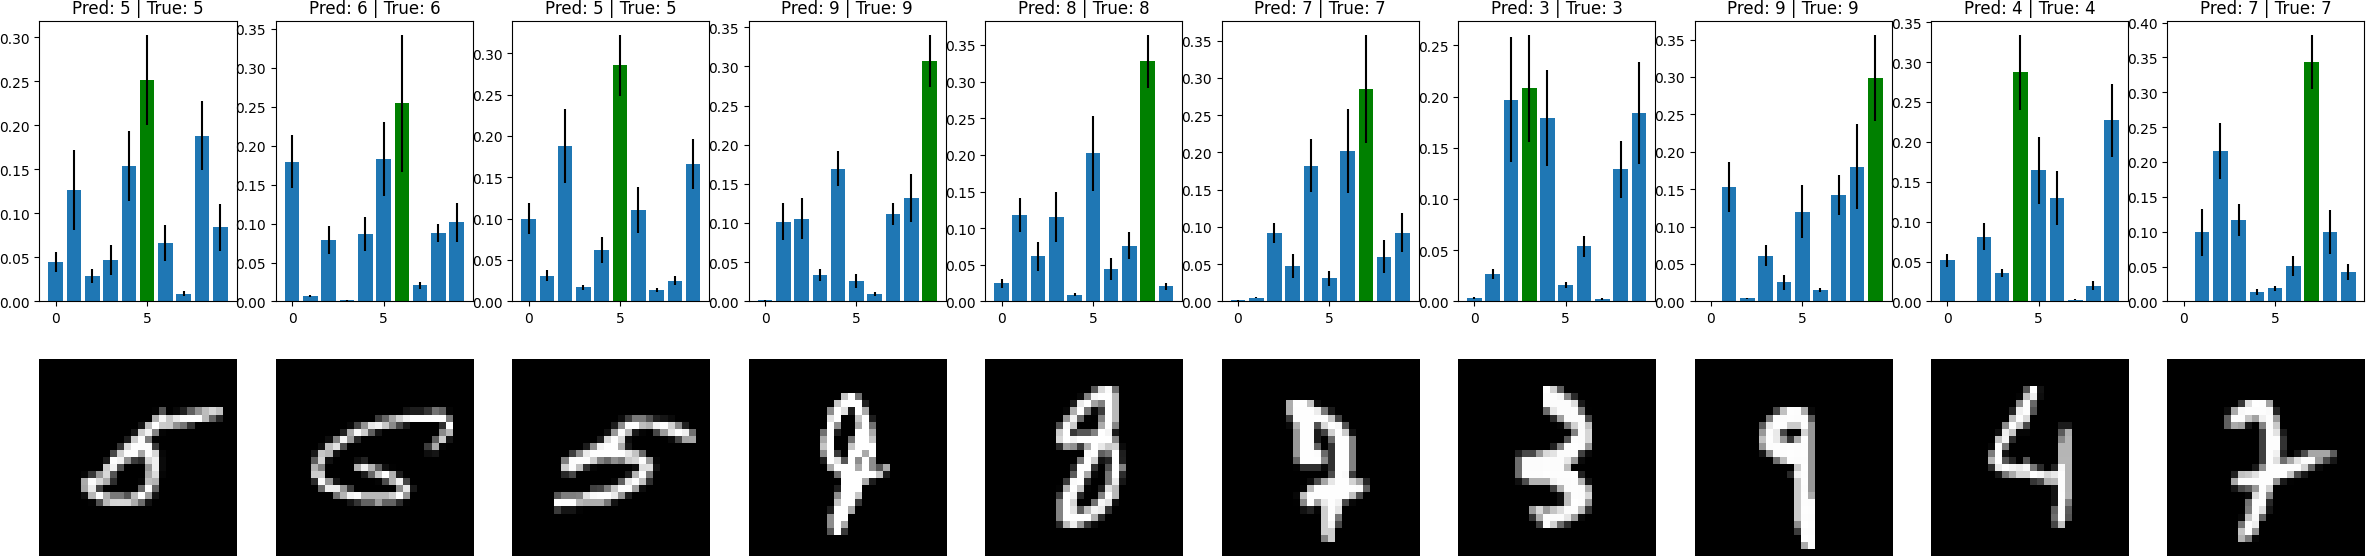
\includegraphics[width=\textwidth]{observational/img/bnn/bnn_top_low_correct.png}
         \caption{Top 10 low confidence correct predictions}
     \end{subfigure}
     \par\bigskip
     \begin{subfigure}[b]{\textwidth}
         \centering
         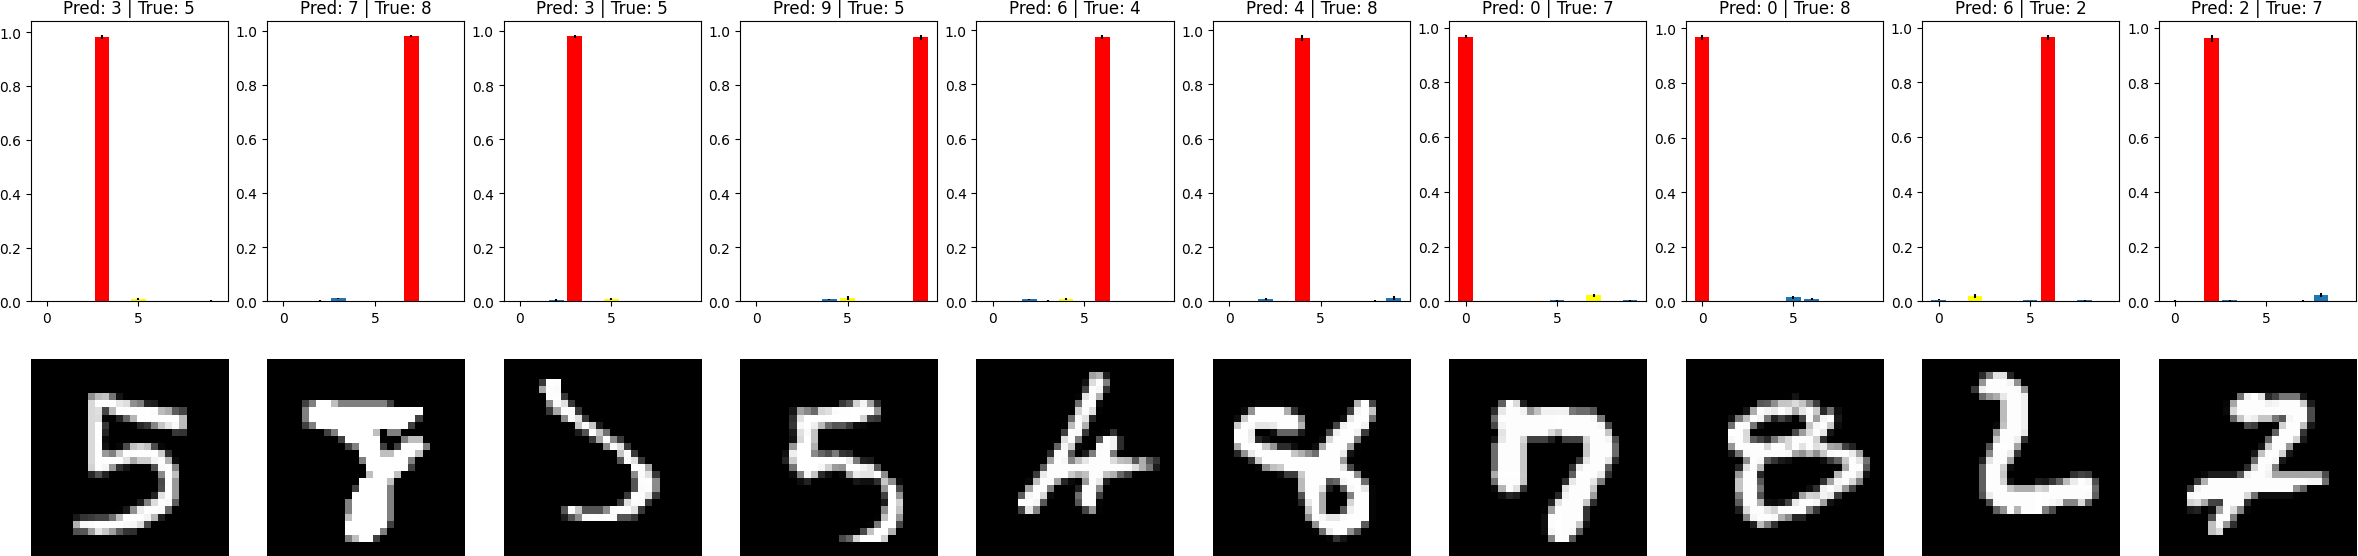
\includegraphics[width=\textwidth]{observational/img/bnn/bnn_top_high_wrong.png}
         \caption{Top 10 high confidence wrong predictions}
     \end{subfigure}
     \par\bigskip
     \begin{subfigure}[b]{\textwidth}
         \centering
         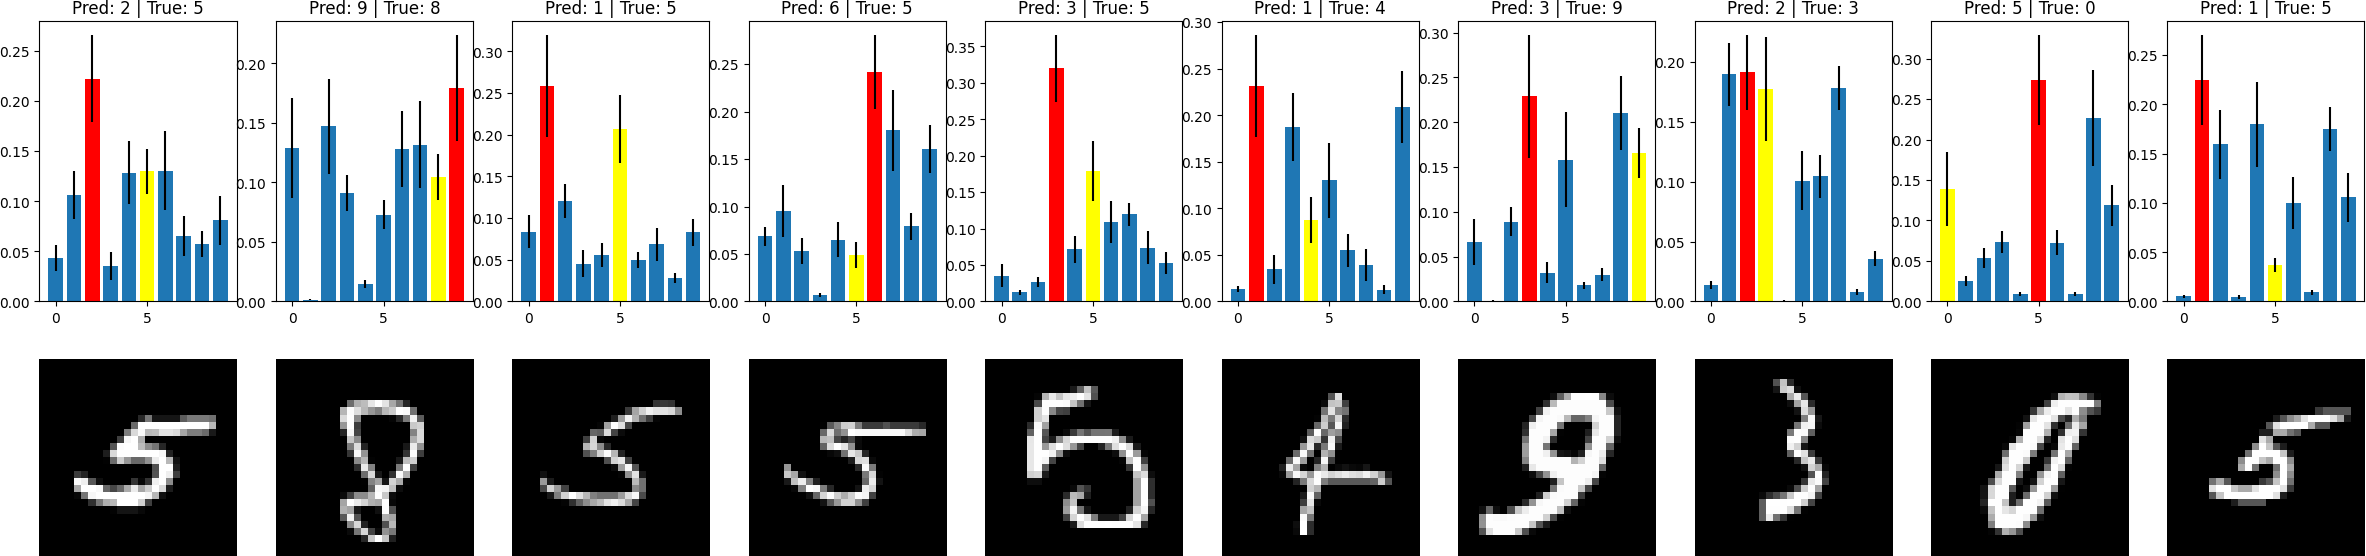
\includegraphics[width=\textwidth]{observational/img/bnn/bnn_top_low_wrong.png}
         \caption{Top 10 low confidence wrong predictions}
     \end{subfigure}
     \caption[Example of uncertainty handling in BNN]{An example of uncertainty handling in Bayesian Neural Networks. Bar plots present correct and wrong predictions with the highest and lowest confidence. Green bars represent confidences in correctly predicted classes, red — confidences in incorrectly predicted classes, yellow — confidence in correct classes in case of an incorrect prediction, blue — confidences in other classes. Bars include \textit{whiskers} to indicate maximum and minimum values over $N=10$ Monte Carlo draws. Below each plot, there is an image of a corresponding sample.}
    \label{fig:bnn-uncertainty}
\end{figure}

\subsection{Prior distributions}
One of the advantages that Bayesian Neural Networks have over the conventional is taking into consideration the prior distribution of weights. Usually, however, the knowledge is vague or non-existent. Thus, a study on sensitivity of the learning to the prior distribution parameters was conducted.

\vspace{\baselineskip}
\autoref{fig:bnn-sigmas} shows loss and accuracy curves for different sigma values. As can be seen, different sigma values do not influence the learning process greatly — the loss decreases and the accuracy increases. The curves are stable for both the train and test batch of data.

\vspace{\baselineskip}
\autoref{fig:bnn-mc} shows loss and accuracy curves for different mixing coefficient values. Similarly to the experiments with sigma parameters, also different proportions of the two distributions do not disrupt the learning process. This is including the two extreme values of $0$ and $1$, where only one of the distribution is active.

% https://tex.stackexchange.com/questions/278727/split-subfigures-over-multiple-pages
\include*{observational/bnn_sigmas}
\include*{observational/bnn_mc}

\vspace{\baselineskip}
While the search was in no way exhaustive, the values used were wide-ranging. Based on the learning curves, a conclusion can be made that even though the parameters of the prior distributions vary, the method is apt to converge.